\documentclass[11pt,a4paper]{article}

% ----- Packages -----
\usepackage[utf8]{inputenc}
\usepackage[T1]{fontenc}
\usepackage{lmodern}
\usepackage[margin=1in]{geometry}
\usepackage{microtype}
\usepackage{setspace}
\usepackage{graphicx}
\usepackage{booktabs}
\usepackage{tabularx}
\newcolumntype{L}{>{\raggedright\arraybackslash}X}
\usepackage{multirow}
\usepackage{threeparttable}
\usepackage{siunitx}
\usepackage{amsmath}
\usepackage{amssymb}
\usepackage{xcolor}
\usepackage[hidelinks,pdfusetitle]{hyperref}
\usepackage{cleveref}
\usepackage{authblk}
\usepackage{titlesec}
\usepackage{caption}
\usepackage{abstract}
\usepackage{orcidlink}

% ----- Typography -----
\setstretch{1.15}
\titleformat{\section}{\normalfont\bfseries\large}{\thesection}{0.7em}{}
\titleformat{\subsection}{\normalfont\bfseries\normalsize}{\thesubsection}{0.6em}{}
\captionsetup[figure]{font=small,labelfont=bf,labelsep=period}
\captionsetup[table]{font=small,labelfont=bf,labelsep=period}

\definecolor{accent}{HTML}{2874A6}
\hypersetup{citecolor=accent, linkcolor=accent, urlcolor=accent}

% ----- Metadata -----
\title{\textbf{The Choice of Data-Lock Anchor Changes Estimated
Post-Completion Endpoint-Amendment Rates 4-fold on ClinicalTrials.gov:
A Methodological Note With a Reusable Pipeline}}

\author[1]{Shizhi Gu\,\orcidlink{0009-0009-3036-2268}\thanks{Correspondence:
\href{mailto:shizhigu97@gmail.com}{shizhigu97@gmail.com}}}
\affil[1]{Independent researcher}

\date{Version 1.0 --- \today}

% ============================================================
\begin{document}
\maketitle

% ----- Abstract -----
\begin{abstract}
\noindent
\textbf{Background.} Registered-primary-outcome changes between trial data
lock and results publication are a form of selective outcome reporting.
Any prevalence estimate for such changes in \texttt{ClinicalTrials.gov}
(CT.gov) depends on the temporal anchor chosen to define ``data lock.''
To our knowledge, no prior audit has quantified how much that choice
matters.

\noindent
\textbf{Objective.} Estimate how the choice of data-lock anchor
(\texttt{ResultsFirstPostDate} vs \texttt{ResultsFirstSubmitDate})
affects the rate of ``post-completion'' primary-outcome amendments in
recently updated Phase~3 industry-sponsored trials on CT.gov.

\noindent
\textbf{Methods.} We sampled the 1{,}000 most-recently-updated
COMPLETED or TERMINATED Phase~3 industry-sponsored trials
(enrolment $\geq 300$) on CT.gov, queried 16~April~2026. For each trial
we retrieved the complete version history through
\texttt{api/int/studies/\{NCT\}/history}---a CT.gov endpoint that
powers the public History tab but is not in the v2 API reference. This
provides live per-trial access to the same historical data the AACT
database aggregates~\cite{aact}. Every meaningful primary-outcome
amendment was classified into temporal windows relative to
\texttt{primary\_completion\_date} and a chosen data-lock anchor.

\noindent
\textbf{Results.} 275/1000 trials (27.5\%, 95\%~CI 24.8--30.3\%) had
at least one meaningful primary-outcome amendment. Classified against
\texttt{ResultsFirstPostDate}, 115/1000 (11.5\%, 95\%~CI 9.7--13.6\%)
fell in the ``between-window'' (primary completion $\rightarrow$
results posting). Replacing the anchor with
\texttt{ResultsFirstSubmitDate} reduced this to 28/1000 (2.8\%,
95\%~CI 1.9--4.0\%)---a 4.1-fold reduction attributable entirely to
anchor choice. Independent case-study verification of three
high-profile candidates (NCT04569084, NCT04738487, NCT03179631)
showed that registry text-level audits are a lower bound: they miss
manipulation at the statistical-analysis-plan (SAP) level.

\noindent
\textbf{Conclusions.} Future systematic audits of registered-outcome
changes should report both anchor variants. Registry text audits
capture only text-level endpoint changes and cannot detect SAP-level
manipulation; they should be viewed as complementary to FDA briefing-
document audits, not a replacement. The audit pipeline is released
under MIT licence.

\medskip
\noindent
\textbf{Keywords:} \texttt{ClinicalTrials.gov}; registered outcome;
primary endpoint; outcome switching; trial integrity; statistical
analysis plan; methodology.
\end{abstract}

% ============================================================
\section{Introduction}

Registration of clinical-trial primary outcomes before enrolment is a
cornerstone of the ICMJE~\cite{icmje2005} and FDAAA~\cite{fdaaa2007,%
fdaaa_final_rule_2016} trial-transparency regime. A registered outcome
that is changed after data lock, but before the trial's results are
made public, is a form of selective outcome reporting known to inflate
effect estimates~\cite{dwan2008outcome,li2018ct_protocol_deviation}.
The \textsc{COMPare} study~\cite{goldacre2019compare} documented
pervasive discrepancies between registered and published outcomes in
67 trials via manual comparison. More recent work
\cite{heneghan2017trialstracker,zarin2019ctgov} has automated
downstream analyses of results posting but has not focused on the
mid-pipeline window in which amendments are most ambiguous:
\emph{after primary completion, before results submission}.

Any prevalence estimate for post-completion primary-outcome changes
requires a temporal anchor for ``data lock.'' Two natural candidates
are exposed by CT.gov's metadata schema:
\begin{itemize}\setlength\itemsep{0.2em}
    \item \texttt{ResultsFirstPostDate}---the date CT.gov \emph{posted} the
          results submission to the public interface;
    \item \texttt{ResultsFirstSubmitDate}---the date the sponsor
          \emph{submitted} the results to CT.gov for review, typically
          several weeks earlier.
\end{itemize}
Sponsors prepare results for submission in a defined internal window
following the primary completion date. Amendments made during this
submission-preparation window are administrative rewording of the
registered outcome to match the final results module, not
manipulation of the endpoint definition itself. Classifying such
changes as ``post-completion manipulation'' over-estimates the
manipulation rate.

In this methodological note we ask: \emph{how much does the choice of
anchor matter?} We audit a 1{,}000-trial cohort from CT.gov and report
rates under both anchors. We also illustrate, with three high-profile
case studies, that text-level registry audits fundamentally cannot
detect manipulation at the statistical-analysis-plan (SAP)
level---a limitation that applies to all prior work in this area as
well as our own. We release the pipeline as open source.

\paragraph{Contributions.}
\begin{enumerate}\setlength\itemsep{0.2em}
    \item Empirical quantification of the anchor-choice sensitivity:
          4.1-fold difference in the estimated ``post-completion''
          amendment rate (from 11.5\% to 2.8\%) across 1{,}000 trials.
    \item A reusable audit pipeline implemented against a
          publicly-accessible CT.gov endpoint (not documented in the
          v2 API reference but mirroring what AACT makes available
          in aggregated form~\cite{aact}), enabling targeted
          per-trial audit without an AACT database clone.
    \item Case-study illustration, via three high-profile trials,
          that text-level audits are a \emph{lower bound} on
          manipulation---SAP-level changes (population switches,
          analysis-method changes) are invisible to registry text
          comparison. This is relevant not only to our pipeline but
          to any prior registry-text audit including COMPare.
\end{enumerate}

% ============================================================
\section{Methods}

\subsection{Data source: CT.gov internal history endpoint}
The CT.gov study page exposes a public ``History of Changes'' tab that
lists every historical revision of the registration. This tab is
populated by two internal endpoints:
\begin{itemize}\setlength\itemsep{0.2em}
    \item \texttt{GET /api/int/studies/\{NCT\}/history} returns a list
          of all versions with \texttt{version}, \texttt{date},
          \texttt{status}, and \texttt{moduleLabels} indicating which
          protocol modules changed in that version.
    \item \texttt{GET /api/int/studies/\{NCT\}/history/\{version\}}
          returns the full protocol and results section for that
          specific historical version.
\end{itemize}
These endpoints are stable and publicly accessible but are not listed
in the CT.gov v2 API reference. The same historical data is available
in aggregated form through the AACT database~\cite{aact}. To verify
that the internal endpoint exposes consistent data with the public
v2 API, we implemented a unit test
(\texttt{tests/test\_api\_agreement.py}) that fetches the latest
version from the internal endpoint and compares the primary-outcome
list to the v2 API's current record for the same trial. All five
tested trials (NCT04006457, NCT04991935, NCT03179631, NCT04738487,
NCT02477800) showed identical primary-outcome sequences. Our
pipeline exists to enable targeted per-trial audit without an AACT
database clone; it is not intended to replace AACT for systematic
work.

\subsection{Cohort}
We queried CT.gov on 16~April~2026 with filters
\texttt{overallStatus=COMPLETED,TERMINATED},
\texttt{Phase=PHASE3}, \texttt{LeadSponsorClass=INDUSTRY},
\texttt{enrollmentCount} $\geq 300$, sorted by
\texttt{LastUpdatePostDate} descending, and retained the first
1{,}000 records.

\subsection{Primary-outcome change classifier}
For every trial we retrieved the subset of versions whose
\texttt{moduleLabels} indicated a change to the Outcome Measures
module, plus \texttt{version 0} (initial registration) and the latest
version. For each adjacent pair we computed the symmetric set
difference of normalised primary-outcome texts.

Normalisation lowercased the text, retained parenthetical abbreviations
(e.g., ``(Cmax)''), stripped common analytic prefixes (``change from
baseline in \ldots''), and expanded a small dictionary of
field-specific acronyms (CDR-SB, ALSFRS-R, PFS, OS, ORR, DoR, PANSS,
MADRS). Two measures were considered the same if either
(a) their content-token Jaccard similarity exceeded 0.5, or
(b) one was a superstring of the other at $\geq 75\%$
content-token containment. Thresholds were fixed \emph{a priori} and
were not calibrated against a labelled ground-truth endpoint-swap
dataset; sensitivity analysis is deferred (see Limitations).

Any outcome added or removed after normalisation was a
\emph{meaningful} change; changes that were detected only as count
shifts (without text shift) were \emph{not} counted.

\subsection{Temporal windows}
Let $c$ be the date of the amendment,
$p$ the trial's \texttt{primaryCompletionDate},
$s$ its \texttt{ResultsFirstSubmitDate}, and
$r$ its \texttt{ResultsFirstPostDate}.
Two anchor conventions were evaluated:

\paragraph{v1 anchor (\texttt{ResultsFirstPostDate}, na\"ive).}
\begin{align*}
    \text{A} &:\ c < p, \\
    \text{B} &:\ p \leq c < r-30\text{d}, \\
    \text{C} &:\ r-30\text{d} \leq c \leq r+30\text{d}.
\end{align*}

\paragraph{v2 anchor (\texttt{ResultsFirstSubmitDate}).}
\begin{align*}
    \text{A} &:\ c < p, \\
    \text{B} &:\ p \leq c < s-7\text{d}, \\
    \text{C} &:\ s-7\text{d} \leq c \leq r+30\text{d}.
\end{align*}

The 7-day buffer before submission is a pragmatic convention to avoid
bordering single-day coincidences; it is not derived from ICMJE or
FDAAA policy. When \texttt{ResultsFirstSubmitDate} was unavailable
(results not yet submitted) we conservatively treated such trials as
uncensored B candidates.

\subsection{Statistical reporting}
Proportions are reported with Wilson 95\%~confidence
intervals~\cite{agresti2002categorical}. Differences between v1 and
v2 B-window rates are reported as raw counts and ratios; no formal
hypothesis test is performed because the comparison is between two
classifiers applied to the same cohort (not two samples).

\subsection{Case-study verification protocol}
Three high-profile candidates from the v1 B-window list
(NCT04569084 Tanabe oral edaravone;
NCT04738487 Merck pembrolizumab/vibostolimab;
NCT03179631 PTC ataluren) were investigated by web search
(press releases, peer-reviewed publications, regulatory documents,
independent trade commentary) to determine whether the registered
change corresponded to a substantive manipulation or to an
administrative amendment. Case-study verification was performed by
a single investigator; no inter-rater assessment is reported. The
three cases are \emph{illustrative}, not a random sample.

% ============================================================
\section{Results}
\label{sec:results}

\subsection{Overall amendment rates}
\Cref{tab:main} summarises the 1{,}000-trial audit. Of all trials,
275 (27.5\%, 95\%~CI 24.8--30.3\%) had at least one meaningful
primary-outcome amendment across their version history.

\begin{table}[htbp]
\centering
\caption{Primary-outcome amendment counts in 1{,}000 Phase~3
industry-sponsored CT.gov trials. Proportions with Wilson
95\%~CI.}\label{tab:main}
\begin{tabular}{lrcc}
\toprule
Window & $n$ & \% of 1{,}000 & 95\%~CI \\
\midrule
Any meaningful change                                & 275 & 27.5 & (24.8, 30.3) \\
A --- pre-completion amendment                       & 132 & 13.2 & (11.2, 15.4) \\
B v1 --- \texttt{ResultsFirstPostDate} anchor        & 115 & 11.5 & (9.7, 13.6)  \\
B v2 --- \texttt{ResultsFirstSubmitDate} anchor      & \textbf{28}  & \textbf{2.8}  & (1.9, 4.0)   \\
C --- results-reporting rewording                    &  83 & \phantom{0}8.3 & (6.7, 10.2)  \\
\bottomrule
\end{tabular}
\end{table}

\subsection{The anchor-choice effect}
The key result is the 4.1-fold difference between the v1 and v2
B-window rates (11.5\% vs 2.8\%, ratio $=4.11$;
\Cref{fig:anchor}). Of the 115 v1 B-hits, 87 (75.7\%, 95\%~CI
66.9--82.6\%) reclassify as C under v2, and 28 (24.3\%) remain in B.

\begin{figure}[htbp]
\centering
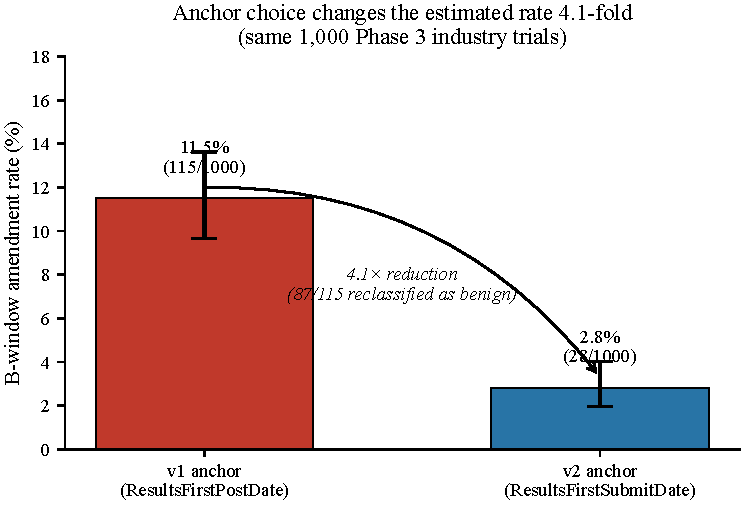
\includegraphics[width=0.82\textwidth]{figures/fig2_anchor_comparison.pdf}
\caption{Estimated B-window amendment rate under the two anchor
conventions. Error bars are Wilson 95\% confidence intervals. The
ratio is deterministic once the cohort is fixed; the difference
captures amendments made during the sponsor's results-submission
preparation window.}\label{fig:anchor}
\end{figure}

The distribution of amendment dates relative to the submission
timestamp (\Cref{fig:dist}) shows the expected pattern: a dense
cluster of text changes in the 0--60 day window immediately
preceding submission, tapering toward the tail. The v2 classifier
assigns the cluster to C (benign rewording during results preparation)
and retains only the sparse long-tail amendments in the B-window.

\begin{figure}[htbp]
\centering
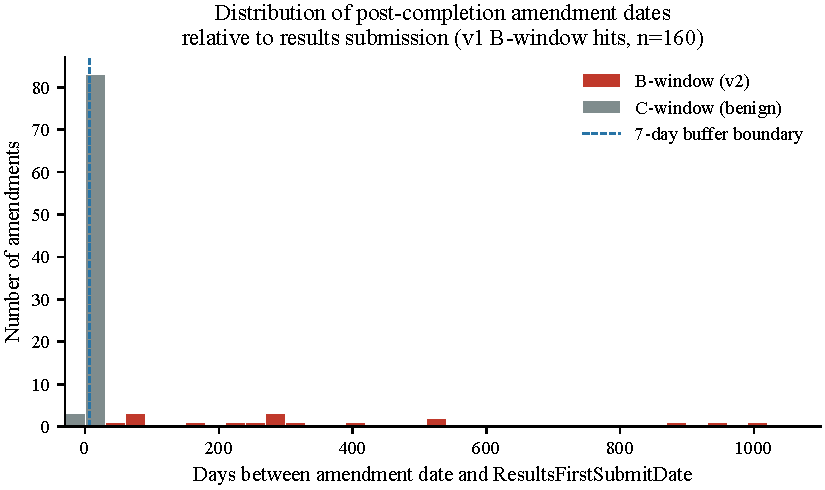
\includegraphics[width=0.85\textwidth]{figures/fig1_distribution.pdf}
\caption{Distribution of meaningful primary-outcome amendment dates
relative to \texttt{ResultsFirstSubmitDate}, across the 160 individual
amendment events contributed by the 115 v1 B-window trials (some
trials contributed more than one amendment event). The
submission-preparation cluster (right-edge red/grey stack) drives
the 4-fold inflation in the v1 rate.}\label{fig:dist}
\end{figure}

This ratio is \emph{deterministic} given the anchor choice; it is not
a random-sample finding. The interpretation is that sponsors amend
registered primary-outcome text during the results-submission
preparation window at a rate that dwarfs genuine post-completion
manipulation, and any audit that classifies such amendments as
``post-completion'' without using a submission-date anchor will
over-estimate the manipulation rate by approximately 4-fold.

\subsection{Three case-study verifications}
Three v1 B-window trials with high public profiles were investigated
to illustrate the interpretive gap between a flagged registry change
and substantive trial manipulation.

\paragraph{NCT04569084 --- Tanabe oral edaravone (ALS).}
Our classifier flagged a primary-outcome change from
\emph{ALSFRS-R at Week~48} to \emph{CAFS at Week~48} in version~56
(2024-11-05). Investigation established that the trial was terminated
for futility on 31~July~2023 on the ALSFRS-R endpoint~\cite{tanabe_mt1186_2024};
final results were presented 17~June~2024 and published
September~2025~\cite{rothstein2025edaravone} reporting both CAFS
(primary) and ALSFRS-R (key secondary), both negative. The registry
amendment post-dated the publication by four months and represents
retroactive alignment of the registration module, not hidden
manipulation. \textbf{Verdict: registry lag; no manipulation.}

\paragraph{NCT04738487 --- Merck pembrolizumab/vibostolimab (KEYVIBE-003).}
Our classifier flagged a primary-outcome collapse from five listed
primaries (PFS and OS across three PD-L1 TPS bins) in version~45 to
one primary (OS in TPS~$\geq 50\%$) in version~136, post primary
completion. Investigation established~\cite{merck_keyvibe_2024}
that the protocol's pre-specified primary was always OS in TPS~$\geq
50\%$; version~45's five-primary listing was an earlier registration
error. Merck announced on 16~December~2024 that the trial stopped
for futility and that the entire vibostolimab programme
(KEYVIBE-003, -006, -007, -008, -010) was discontinued.
\textbf{Verdict: registry error correction; no manipulation.}

\paragraph{NCT03179631 --- PTC ataluren (Duchenne muscular dystrophy,
Study~041).}
Our classifier flagged an expansion from one primary outcome
(\emph{slope of 6MWD change over 72 weeks}) in version~10 to four
primaries (ITT vs mITT $\times$ change vs average rate) in version~50,
3.8 years after primary completion. Investigation established that
the published paper~\cite{ptc_muntoni_2025} reports one primary
(slope in ITT, $p=0.0248$), and the four-endpoint listing reflects
CT.gov results-module formatting rather than a scientific re-analysis.
However, a substantive manipulation did occur at a layer our pipeline
cannot see: the statistical analysis plan's pre-specified analysis
\emph{population} was switched between earlier submissions and the
final analysis. The FDA's reviewing division withdrew the NDA
resubmission on 13~February~2026 stating that the data were
``unlikely to show enough efficacy to support regulatory
approval''~\cite{ptc_withdrawal_2026}; the EMA finalised
non-renewal of the conditional marketing authorisation on
28~March~2025. \textbf{Verdict: registry text change cosmetic; real
manipulation occurred at the SAP level and was invisible to
text-level registry audit.}

% ============================================================
\section{Discussion}

\subsection{What this study establishes}
The choice of data-lock anchor produces a 4.1-fold spread in the
estimated rate of ``post-completion'' primary-outcome amendments.
Using \texttt{ResultsFirstPostDate} conflates genuine post-completion
changes with administrative rewording in the results-submission
preparation window; using \texttt{ResultsFirstSubmitDate} separates
the two. The 2.8\% v2 rate is our best per-trial estimate of amendment
activity in the submission-preparation and post-submission window,
limited to the exact sampled population (recently-updated, recent-era,
large Phase~3 industry trials).

\subsection{What this study does not establish}
The 2.8\% figure is \emph{not} a manipulation rate. A single-rater
review of the three highest-profile v2 candidates found two registry-
lag cases and one that masked substantive manipulation at a layer
invisible to registry text comparison. A defensible manipulation
rate requires (a)~a random sample of flagged cases, (b)~blinded
adjudication by at least two independent raters, (c)~pre-registered
triage criteria, and (d)~cross-reference to FDA briefing documents.
These are appropriate targets for a follow-up study.

\subsection{Generalisability}
Our cohort was sorted by \texttt{LastUpdatePostDate} descending. This
biases the sample toward recent, actively-maintained registrations
(2023--2026 era). Generalisability to older trials, to trials that
stopped updating after results posting, or to non-industry sponsors
is unknown. A random-sample replication stratified by completion
year is a natural extension.

\subsection{Relation to prior work}
\textsc{COMPare}~\cite{goldacre2019compare} compared 67 trials'
registrations to their publications by manual inspection and found
frequent outcome switching. Chen et al.~\cite{chen2016bmj} analysed
results publication across academic medical centers.
Zarin et al.~\cite{zarin2019ctgov} reported on a decade of results
submission to CT.gov. Our study differs in scope and unit of analysis:
we compare registration versions to each other across 1{,}000
trials and do not attempt registration-vs-publication comparison. The
methods are complementary. AACT~\cite{aact} exposes the same
historical registration data we use, but as a relational database
clone; our pipeline exists to enable targeted per-trial queries
without local database setup, not to replace AACT's systematic
infrastructure.

\subsection{Limitations}
\begin{enumerate}\setlength\itemsep{0.2em}
    \item Sampling by \texttt{LastUpdatePostDate} over-represents
          conscientious sponsors.
    \item Case-study verification was performed by a single investigator
          without inter-rater reliability measurement.
    \item Similarity thresholds (Jaccard 0.5, superstring 0.75)
          were not calibrated against a ground-truth endpoint-swap
          dataset; sensitivity analysis is deferred.
    \item \texttt{primaryCompletionDate} values used for the
          A/B classification were the current-API values, not the
          historical values at each amendment time. Retrospective
          amendments to the completion date itself could shift the
          classification (Goldacre et al. document this
          practice~\cite{goldacre2019compare}).
    \item The 7-day buffer before \texttt{ResultsFirstSubmitDate} is
          pragmatic, not policy-grounded.
    \item Text-level registry audits cannot detect
          statistical-analysis-plan (SAP) changes such as
          population switches or analysis-method changes. Complete
          manipulation detection requires access to SAP documents
          or FDA briefing materials.
\end{enumerate}

\subsection{Recommendations for future audits}
\begin{itemize}\setlength\itemsep{0.2em}
    \item Report both anchor variants, not just one.
    \item Use \texttt{ResultsFirstSubmitDate}, where available, as the
          primary anchor; fall back to \texttt{ResultsFirstPostDate}
          only when submission date is unreported.
    \item Combine registry-text auditing with SAP-level auditing
          (FDA briefing documents where available).
    \item Pre-register triage criteria, sample size, and inter-rater
          assessment protocol before extending beyond the proof-of-
          concept stage.
\end{itemize}

\section*{Data and code availability}
All audit code and classifier implementation are available at
\url{https://github.com/shizhigu/ct-endpoint-audit} under the MIT
licence. The full 1{,}000-trial audit output (JSON with per-version
primary-outcome diffs and per-trial metadata) is archived on Zenodo
(DOI to mint at submission time). The CT.gov internal history endpoint
is accessed without authentication at
\texttt{https://clinicaltrials.gov/api/int/studies/\{NCT\}/history}.

\section*{Conflicts of interest}
The author declares no competing interests. This research was unfunded.

\section*{Acknowledgements}
Automated critique tooling was used during manuscript preparation to
identify methodological weaknesses in an earlier draft, including
the tautological headline claim, the over-claimed ``undocumented
API'' contribution, and the selection-bias issue in the sampling
frame. The final text reflects those revisions.

\bibliographystyle{unsrt}
\bibliography{references}

\clearpage
\appendix

\section*{Supplementary Materials}

% Supplementary Table S1
% Auto-generated from data/r23_reclassified_v2.json
\begin{table}[htbp]
\centering
\caption{Supplementary Table S1. The 28 trials flagged as B-window
(locked-data, pre-submission) under the refined anchor. Sorted by
primary completion date (most recent first). \emph{(none)} in the
\emph{Results-first submitted} column indicates results not yet
submitted at query time; such trials remain B-window candidates
pending future data.}\label{tab:s1}
\footnotesize
\begin{tabularx}{\textwidth}{@{}l L l l l@{}}
\toprule
NCT & Sponsor & Primary & Results-first & Change \\
    &         & completion & submitted & date \\
\midrule
NCT06284915 & Sanofi Pasteur, a Sanofi Company & 2025-11-14 & (none) & 2025-11-24 \\
NCT05842954 & Novartis Pharmaceuticals & 2025-06-27 & (none) & 2025-12-11 \\
NCT06553456 & Protgen Ltd & 2025-05-14 & (none) & 2025-09-24 \\
NCT05811247 & Apnimed & 2025-05-07 & (none) & 2025-11-18 \\
NCT05997290 & BioNTech SE & 2025-03-13 & (none) & 2026-03-09 \\
NCT05813275 & Apnimed & 2025-03-10 & (none) & 2025-11-18 \\
NCT05743075 & Nuance Pharma (shanghai) Co., Ltd & 2024-12-06 & (none) & 2026-01-26 \\
NCT04738487 & Merck Sharp \& Dohme LLC & 2024-09-05 & 2025-07-28 & 2024-10-28 \\
NCT04777201 & Hoffmann-La Roche & 2024-09-03 & 2025-09-02 & 2024-12-06 \\
NCT04770220 & Alzheon Inc. & 2024-05-29 & 2025-09-11 & 2024-07-31 \\
NCT05648110 & AstraZeneca & 2024-03-29 & (none) & 2025-09-25 \\
NCT05573464 & AstraZeneca & 2024-03-26 & 2025-09-02 & 2025-03-25 \\
NCT05142774 & Organon and Co & 2024-02-29 & 2025-01-13 & 2024-04-05 \\
NCT03608033 & Omeros Corporation & 2024-01-12 & 2025-01-10 & 2024-03-12 \\
NCT04432831 & Hoffmann-La Roche & 2023-10-11 & 2024-10-07 & 2024-08-23 \\
NCT06437626 & Pharmasoft & 2023-08-18 & 2025-04-04 & 2024-07-12 \\
NCT02807636 & Hoffmann-La Roche & 2022-08-31 & 2023-08-22 & 2023-06-08 \\
NCT03083665 & UCB Biopharma SRL & 2022-06-30 & 2022-12-15 & 2022-10-06 \\
NCT04478084 & Sanofi Pasteur, a Sanofi Company & 2022-03-19 & (none) & 2022-03-31 \\
NCT05062330 & Aldeyra Therapeutics, Inc. & 2022-03-04 & 2025-02-27 & 2022-06-03 \\
NCT03783442 & BeiGene & 2022-02-28 & 2023-10-10 & 2022-04-26 \\
NCT02967692 & Novartis Pharmaceuticals & 2020-08-11 & 2023-06-26 & 2022-01-14 \\
NCT02017717 & Bristol-Myers Squibb & 2019-06-17 & 2022-06-02 & 2020-01-09 \\
NCT01358877 & Hoffmann-La Roche & 2016-12-19 & 2017-12-04 & 2017-04-20 \\
NCT02677298 & Croma-Pharma GmbH & 2016-11-23 & 2024-12-17 & 2022-05-13 \\
NCT01084876 & Celltrion & 2012-07 & 2024-10-29 & 2024-08-27 \\
NCT00460512 & Janssen-Cilag International NV & 2009-01-22 & (none) & 2009-03-12 \\
NCT00087776 & American Regent, Inc. & 2007-10-27 & (none) & 2025-07-21 \\
\bottomrule
\end{tabularx}
\end{table}


\end{document}
